\chapter{Resultados e discussões sobre as técnicas de metamodelagem}\label{chap_aplicacao}

Verificada a existência de uma enorme gama de metamodelos, alguns deles serão avaliados a seguir considerando funções matemáticas e o prolongamento temporal das respostas de vibração de um \textit{riser} submerso. Como mencionado, o pacote SMT foi utilizado para determinar os resultados deste relatório parcial. Os seguintes metamodelos estão disponíveis nesta biblioteca Python \cite{BOUHLEL2019}:

	\begin{itemize}
	\item KRG - \textit{Kriging};
	\item RBF - \textit{Radial basis functions};
	\item IDW - \textit{Inverse-distance weighting};
	\item RMTS - \textit{Regularized minimal-energy tensor-product splines};
	\item LS - \textit{Least-squares approximation};
	\item QP - \textit{Second-order polynomial approximation};
	\item KPLS - \textit{Kriging model and partial least squares}; 
	\item KPLSK - \textit{Kriging model and partial least squares with gradient}; 
	\item GEKPLS - \textit{Gradient-enhaced Kriging with partial least squares approach};
	\item GENN - \textit{Gradient-enhaced neural network}.
	
\end{itemize}

Em relação aos métodos de amostragem, o SMT tem disponível os seguintes métodos:

\begin{itemize}
\item LHS - \textit{Latin hypercube sampling};
\item \textit{Random sampling};
\item \textit{Full-factorial sampling}.
\end{itemize}

O SMT possui como padrão o método de otimização \textit{Constrained Optimization by Linear Approximations} (COBYLA) desenvolvido por \citeonline{powell1994}. No entanto, existe a possibilidade de utilizar outros métodos clássicos ou evolutivos \cite{scipy}:


\begin{itemize}

	\item \textit{{\color{red}Nelder-mead}};

	\item \textit{Powell};

	\item \textit{Gradient conjugate};

	\item BFGS - \textit{Broyden–Fletcher–Goldfarb–Shanno};

	\item DE - \textit{Differential evolution}.

\end{itemize}

Ainda destaca-se que no SMT existe uma biblioteca de problemas analíticos e de engenharia que estão disponíveis para testar a precisão dos metamodelos implementados. Alguns dos problemas são:

\begin{itemize}
	\item \textit{Sphere};
	\item \textit{Rosenbrock};
	\item \textit{Cantilever-beam}.
\end{itemize}

Ressalta-se que a prática de normalização é comum no contexto da metamodelagem, onde os dados de entrada e saída devem ser normalizados. Para tal, são utilizados a média e o desvio-padrão estimados a partir do conjunto de dados amostrais \cite{SICCHIERI2019}. \textcolor{red}{Esta} estratégia é largamente utilizada com o objetivo de obter os valores com a mesma ordem de grandeza. Por exemplo, um componente de $x$ pode representar uma proporção de Poisson adimensional de alguma liga de aço cuja ordem de grandeza é $0.3$, enquanto outro pode representar o módulo de elasticidade expresso em MPa cuja ordem de grandeza é $2 x 10^{11}$. Logo, esta estratégia de normalização apresentada por \citeonline{lophaven2002}, \citeonline{HWANG2018} e \citeonline{SICCHIERI2019} é usada nos resultados apresentados neste relatório parcial.

Neste contexto, os metamodelos {\it Kriging} e RBF são utilizados neste trabalho. Para o \textit{Kriging}, são consideradas as funções de correlação gaussiana e, posteriormente, a exponencial (GAUSS e EXP, respectivamente). Além disso, o {\it Kriging} comum (OK; polinômio constante) e o universal (UK) são aplicados. No caso do UK, são utilizados os polinômios de primeiro e segundo graus (PG e SG, respectivamente). Para a RBF, são considerados na sua formulação um valor constante (C) e um polinômio linear (LIN). Diferentes números de amostras são usados para o treinamento e validação do metamodelo. Os resultados são avaliados a partir das métricas RMSE e $R^2$.

\section{Função Branin-Hoo}

A função Branin-Hoo é definida por \cite{YIN2018}:
\begin{equation}
y = \left({x_2}-\frac{5.1} {4{\pi}^2}{x_1}^2+\frac{5} {\pi}{x_1}-6\right)^2+10 \left(1-\frac{1} {8\pi}\right)\cos({x_1})+10
\end{equation}

\noindent onde ${x_1} \in [-5,10]$ e ${x_2} \in [0,15]$. A Fig. \ref{fig:branin} mostra o comportamento da função Branin-Hoo dentro do intervalo de amostragem definido.

\begin{figure}[H]
	\centering
	{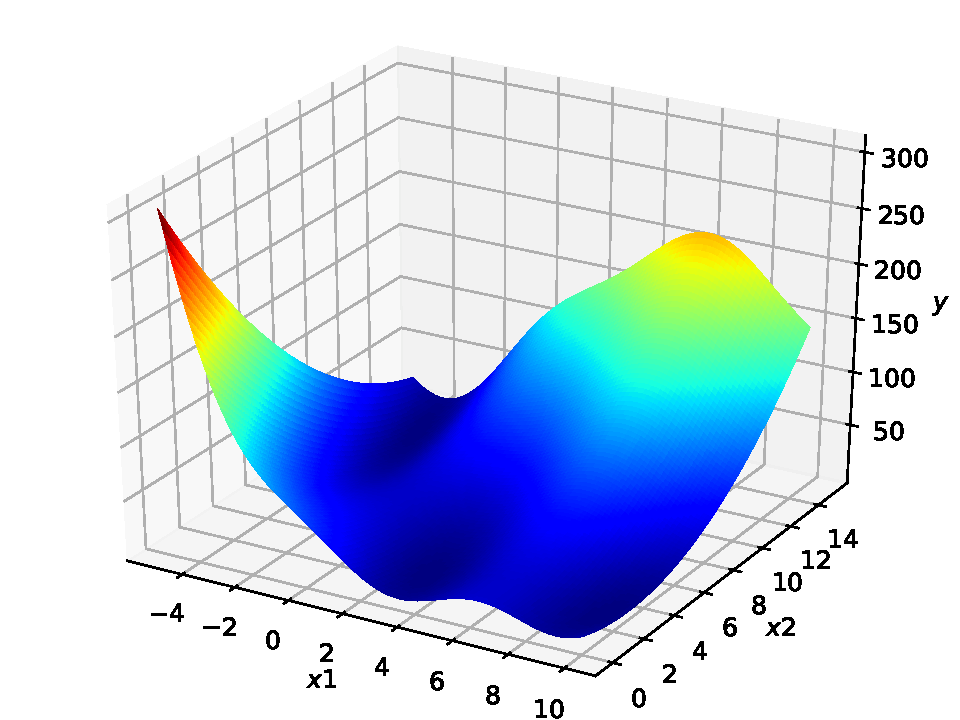
\includegraphics[width= 0.7\linewidth]{tatiane/fig_tati/branin/orig}}
	\caption{Função Branin-Hoo.} 
	\label{fig:branin}
\end{figure}

As Tabs. \ref{1b} e \ref{tab:4} apresentam os resultados obtidos a partir dos métodos {\it Kriging} e RBF considerando diferentes números de amostras obtidas a partir do LHS, a saber: 10, 20, 30, 40, 50 e 60. A validação dos metamodelos foi realizada considerando 1024 amostras adicionais determinadas a partir do método {\it grid} regular. Para tal comparação, \textcolor{red}{calcularam-se} os valores das métricas RMSE e ${R}^2$. Neste caso, foram considerados os valores iniciais $\theta=0.01$ e $\theta=5$ para os métodos {\it Kriging} e RBF, respectivamente. 

É possível observar que o valor RMSE diminuiu a medida que o número de amostras usadas para gerar os metamodelos aumentou. O valor da métrica $R^2$ aumentou de acordo com o número de amostras, evidenciando o aumento da representatividade dos metamodelos obtidos. Desta forma, o metamodelo que melhor representou a função Branin-Hoo dentro do intervalo de amostragem considerado foi o UK-SG-GAUSS.

Para esta função teste, a função de correlação gaussiana mostrou-se mais adequada que a exponencial para o metamodelo {\it Kriging}. Com 30 amostras, o {\it Kriging} conseguiu uma boa representação da resposta, enquanto que a RBF necessitou de mais amostras.

\begin{table}[H]
	\centering
	\caption{Métricas de precisão para a função Branin-Hoo considerando 10, 20 e 30 amostras.} \label{1b} 
	\begin{tabular}{c c c c c c c c c}
		\toprule
		& \multicolumn{2}{c}{\bf 10 amostras} & \multicolumn{2}{c}{\bf 20 amostras} & \multicolumn{2}{c}{\bf 30 amostras} \\ \midrule
		{\bf Metamodelo} & RMSE & {\bf $R^{2}$} & RMSE & {\bf $R^{2}$} & RMSE & {\bf $R^{2}$} \\
		\hline \\
		{OK-GAUSS} & 20.8745 & 0.999858 & 6.7246 & 0.999985 & 2.9782 & 0.999997 \\[4pt]
		OK-EXP & 40.8839 & 0.999455 & 30.6543 & 0.999693 & 34.6247 &	0.999609 \\[4pt]                   
		UK–LIN-GAUSS & 25.4212 & 0.999789 & 11.1048 &	0.999959 & 2.2087 &	0.999998 \\[4pt]
		UK–LIN-EXP & 41.8692 & 0.999429 & 36.5724 & 0.999564 & 36.1190 &	0.999575 \\[4pt]
		UK–SG-GAUSS & 32.9299 & 0.999646 & 5.3233 & 0.999990 & 2.6899 & 0.999997 \\[4pt]
		UK–SG-EXP & 34.1750	& 0.999619 & 21.1318 & 0.999854 & 31.2668	& 0.999681 \\[4pt]
		RBF-C-GAUSS & 28.4381 & 0.999736 & 26.2992 & 0.999774 & 24.7319 &	0.999800 \\[4pt]
		RBF-LIN-GAUSS & 32.7091 & 0.999651 & 27.2394 &	0.999758 & 24.6521 &	0.999802 \\[4pt] \bottomrule
		
	\end{tabular}
	
\end{table}


\begin{table}[H]
	\centering
	\caption{Métricas de precisão para a função Branin-Hoo considerando 40, 50 e 60 amostras.} \label{tab:4} 
	\begin{tabular}{c c c c c c c c c}
		\toprule
		& \multicolumn{2}{c}{\bf 40 amostras} & \multicolumn{2}{c}{\bf 50 amostras} & \multicolumn{2}{c}{\bf 60 amostras} \\ \midrule
		{\bf Metamodelo} & RMSE & {\bf $R^{2}$} & RMSE & {\bf $R^{2}$} & RMSE & {\bf $R^{2}$} \\
		\hline \\
		{OK-GAUSS} & 0.0149 & 0.999999  & 0.0099 & 0.999999 & 0.0100 & 0.999999 \\[4pt]
		OK-EXP & 12.9703 &	0.999945 & 15.3978 & 0.999922 & 7.3084 & 0.999982  \\[4pt]                   
		UK–LIN-GAUSS & 0.0282 &	0.999999 & 0.0092 &	0.999999 & 0.0098 & 0.999999  \\[4pt]
		UK–LIN-EXP & 12.7812 &	0.999946 & 16.8734 & 0.999907 & 7.6077	& 0.999981  \\[4pt]
		UK–SG-GAUSS & 0.0069 & 0.999999 & 0.0043 &	0.999999 & 0.00085 & 0.999999 \\[4pt]
		UK–SG-EXP & 10.1908	& 0.999966 & 11.2550 & 0.999958 & 8.4088 & 0.999976  \\[4pt]
		RBF-C-GAUSS & 4.8563 & 0.999992 & 4.7391 & 0.999992  & 1.3326 & 0.999999 \\[4pt]
		RBF-LIN-GAUSS & 5.8386 & 0.999988 & 2.7598 & 0.999997 & 1.7206 & 0.999999  \\[4pt] \bottomrule
		
	\end{tabular}
	
\end{table}

A Fig. \ref{fig:branin1} mostra o comportamento dos melhores metamodelos formulados para representar a função Branin-Hoo de acordo com o número de amostras geradas pelo LHS. Note que a forma da função é adequadamente representada em todos os casos apresentados. Claramente, existe uma dificuldade dos metamodelos em descrever o comportamento da função Branin-Hoo em suas extremidades (valores maiores de $y$). No entanto, essa dificuldade diminui \textcolor{red}{à} medida que um maior número de amostras é utilizado na formulação dos metamodelos.

\begin{figure}[H]
	\centering
	\subfigure[][]{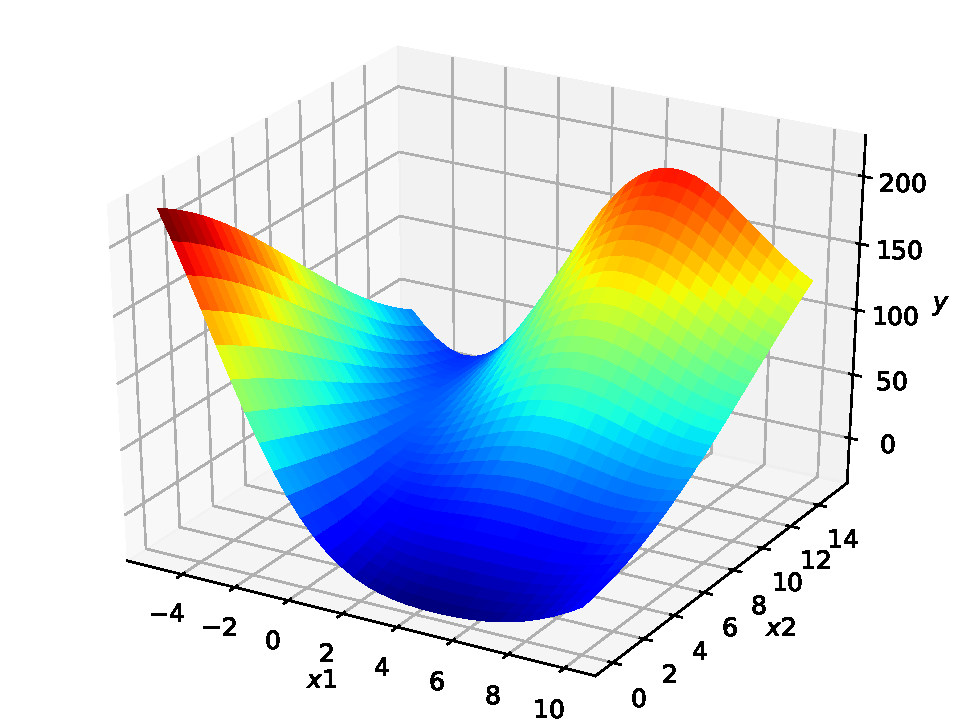
\includegraphics[width=0.47\linewidth]{tatiane/fig_tati/branin/ok.pdf}\label{a}} 
	\subfigure[][]{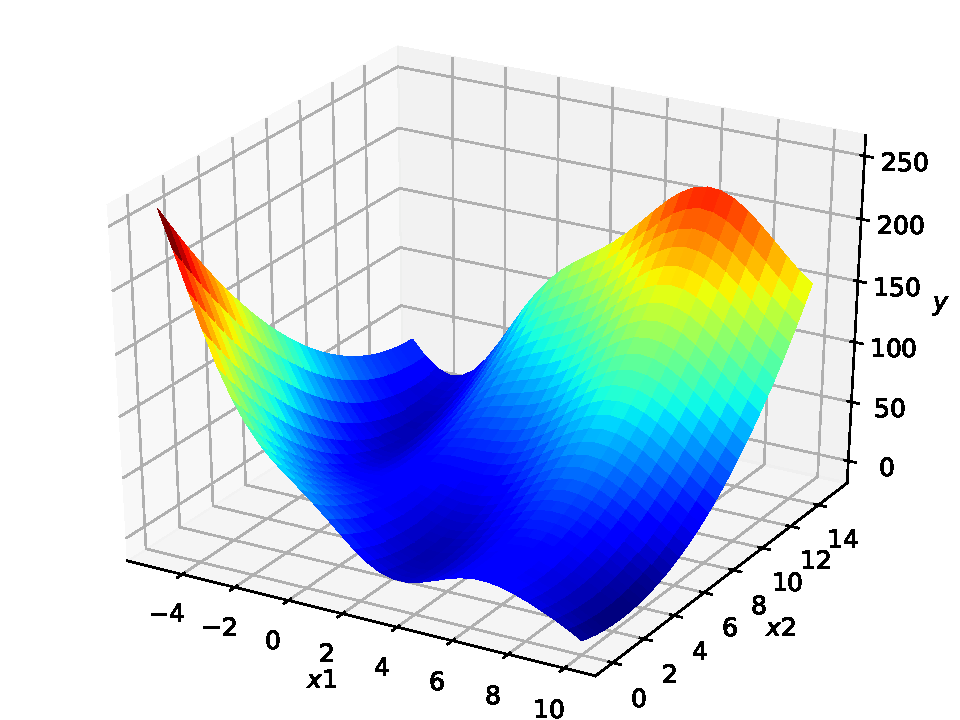
\includegraphics[width=0.47\linewidth]{tatiane/fig_tati/branin/SQGaus.pdf}\label{b}} 
	\subfigure[][]{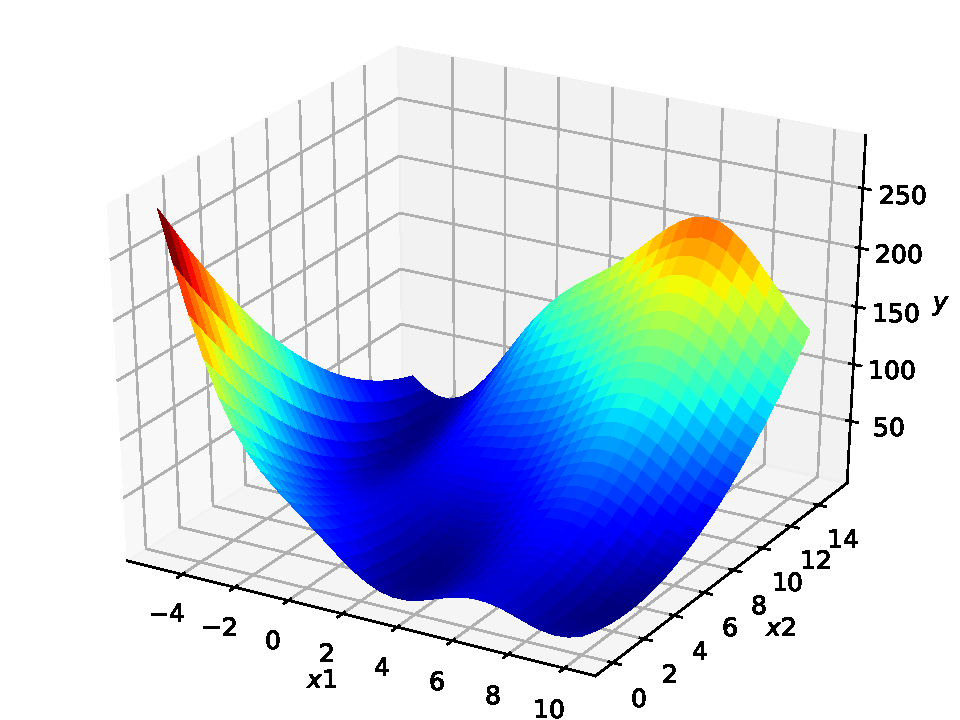
\includegraphics[width=0.47\linewidth]{tatiane/fig_tati/branin/lingaus.pdf}\label{c}} 
	\subfigure[][]{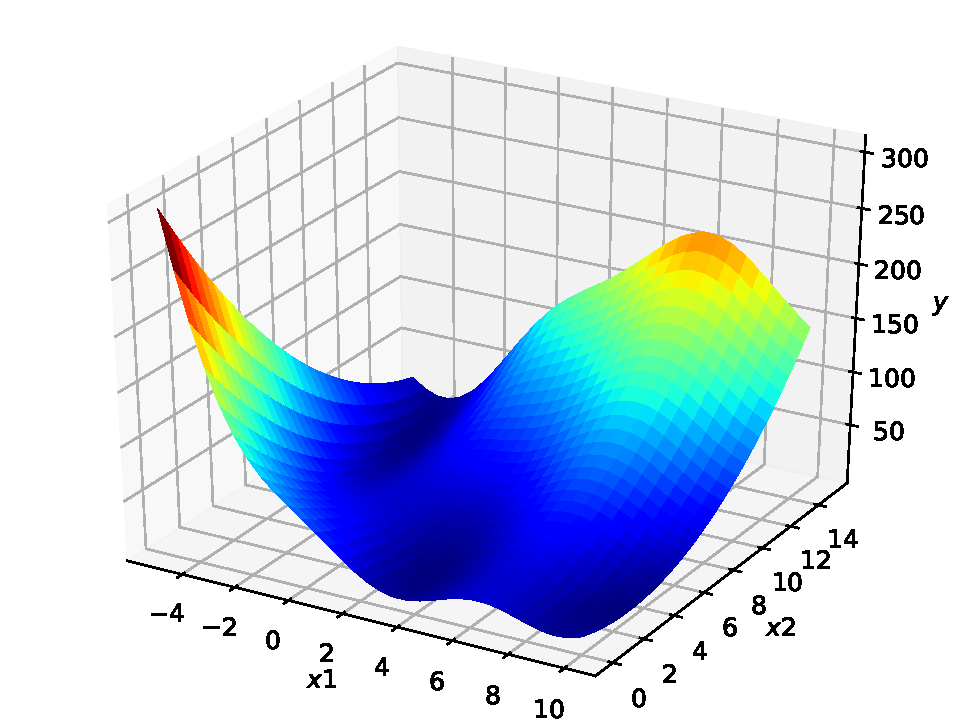
\includegraphics[width=0.47\linewidth]{tatiane/fig_tati/branin/fig4_SQG.pdf}\label{d}} 
	\subfigure[][]{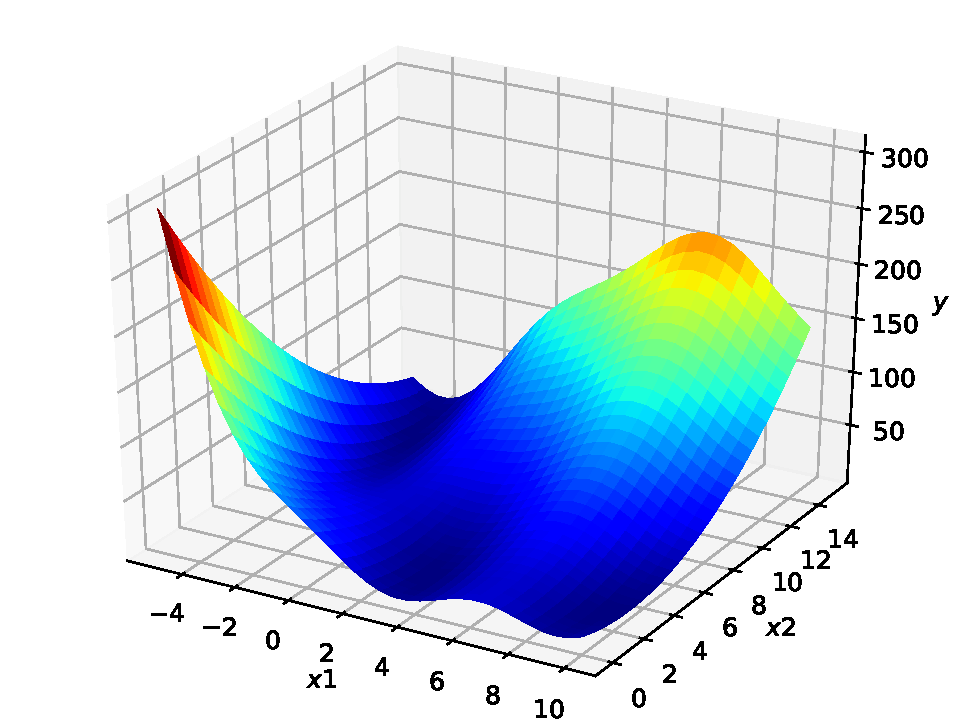
\includegraphics[width=0.47\linewidth]{tatiane/fig_tati/branin/fig5_SQG.pdf}\label{e}} 
	\subfigure[][]{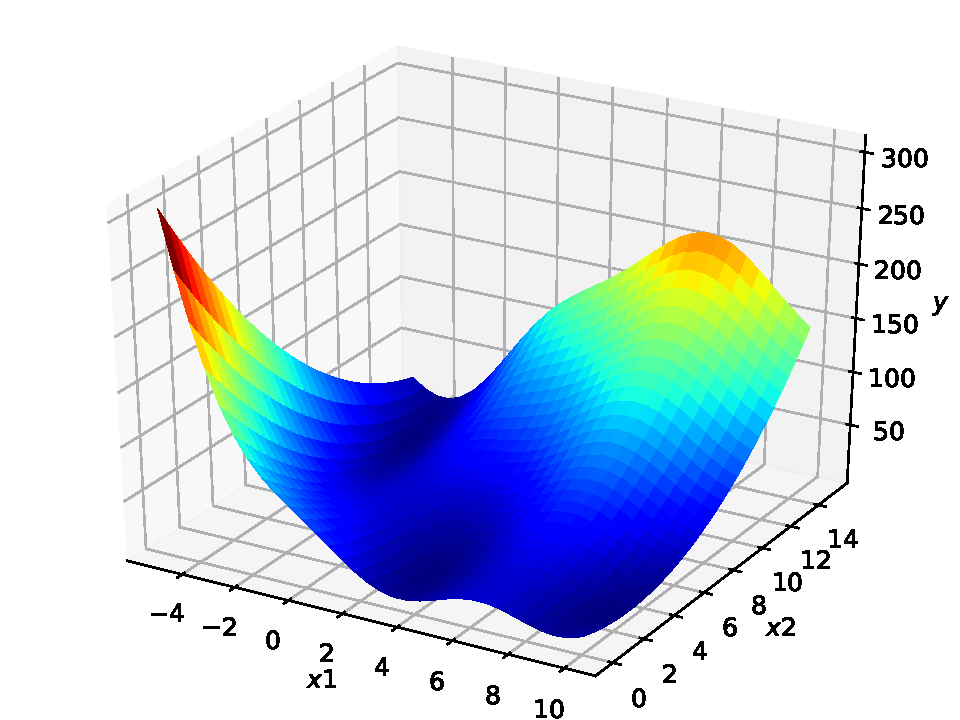
\includegraphics[width=0.47\linewidth]{tatiane/fig_tati/branin/fig6_SQG.pdf}\label{f}} 
	\caption{Melhores configurações para a função Branin-Hoo: a) OK-GAUSS para 10 amostras; b) UK-SG-GAUSS para 20 amostras; c) UK-LIN-GAUSS para 30 amostras; d) UK-SG-GAUSS para 40 amostras; d) UK-SG-GAUSS para 50 amostras; e) UK-SG-GAUSS para 60 amostras.} 
	\label{fig:branin1}
\end{figure}

\section{Função quadrática}

 Outra função teste é encontrada no trabalho de \citeonline{SICCHIERI2019}. Esta função é dada por:
 % equação
 \begin{equation}
 y= \left(30+{x_1}sen{(x_1)}\right)\left(4+\exp(-0.5{x_2}-1)^2 \right)
 \label{eq: 40}
 \end{equation}
 
 \noindent onde ${x_1} \in [-5,\hspace{0.1 cm}5]$ e ${x_2} \in [-5,\hspace{0.1 cm}5]$. A Fig. \ref{fig:leo} mostra o comportamento da função quadrática dentro do intervalo de amostragem definido.
  
 \begin{figure}[H]
 	\centering
 	{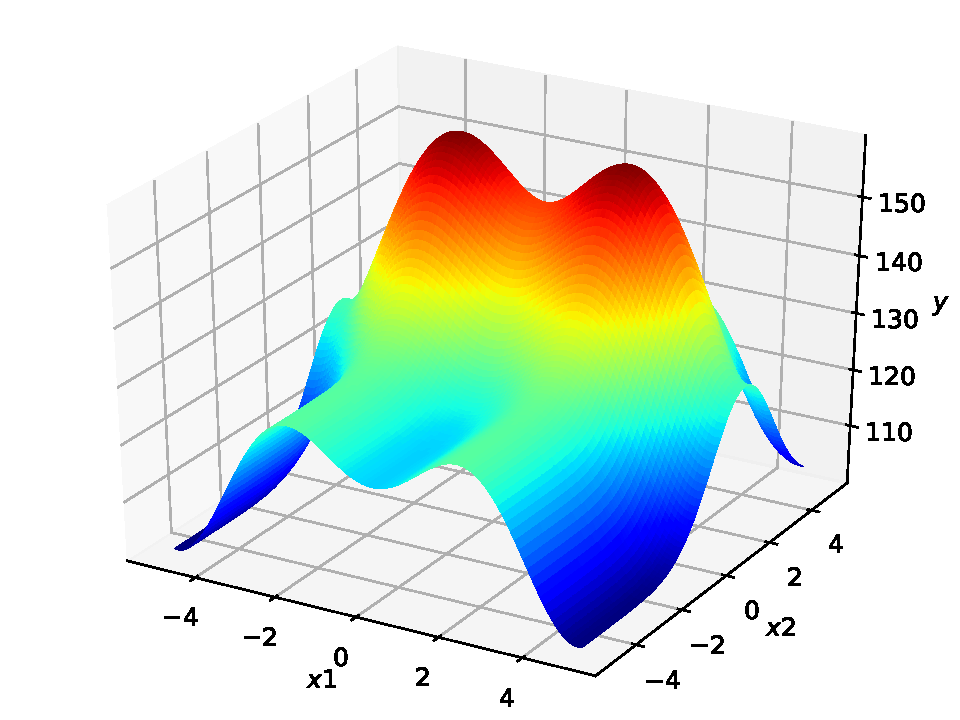
\includegraphics[width=0.7\linewidth]{tatiane/fig_tati/func_leo/fig2_orig.pdf}} 
 	\caption{Função quadrática.} 
 	\label{fig:leo}
 \end{figure}

As Tabs. \ref{tab:5} e \ref{tab:6} apresentam os resultados obtidos a partir dos métodos {\it Kriging} e RBF considerando diferentes números de amostras obtidas a partir do LHS, a saber: 10, 20, 30, 40, 50 e 60. A validação dos metamodelos foi realizada considerando 1024 amostras adicionais determinadas a partir do método {\it grid} regular. Para tal comparação, \textcolor{red}{calcularam-se} os valores das métricas RMSE e ${R}^2$. Como no caso anterior, foram considerados os valores iniciais $\theta=0.01$ e $\theta=5$ para os métodos {\it Kriging} e RBF, respectivamente. 

\begin{table}[H]
	\centering
	\caption{Métricas de precisão para a função quadrática considerando 10, 20 e 30 amostras.} \label{tab:5} 
	\begin{tabular}{c c c c c c c c c}
		\toprule
		& \multicolumn{2}{c}{\bf 10 amostras} & \multicolumn{2}{c}{\bf 20 amostras} & \multicolumn{2}{c}{\bf 30 amostras} \\ \midrule
		{\bf Metamodelo} & RMSE & {\bf $R^{2}$} & RMSE & {\bf $R^{2}$} & RMSE & {\bf $R^{2}$} \\
		\hline \\
		{OK-GAUSS} & 12.0727 & 0.999990 & 6.5667 & 0.999997 & 4.8015 &	0.999998 \\[4pt]
		OK-EXP & 12.8429 & 0.999989 & 4.7737 & 0.999998 & 2.7240 & 0.999999 \\[4pt]                 
		UK–LIN-GAUSS & 7.5362 & 0.999996 & 7.9488 &	0.999995 & 5.0155 & 0.999998  \\[4pt]
		UK–LIN-EXP & 13.1985 & 0.999988 & 4.7107 & 0.999998 & 2.7404 & 0.999999  \\[4pt]
		UK–SG-GAUSS  & 8.2353 & 0.999995  & 5.8390 & 0.999997 & 17.4569 & 0.999980 \\[4pt]
		UK–SG-EXP & 8.6918 & 0.999995 & 5.7322 & 0.999997 & 2.4217	& 0.999999 \\[4pt]
		RBF-C-GAUSS & 9.1103 & 0.999994 & 5.6298 & 0.999997 & 4.8492 & 0.999998  \\[4pt]
		RBF-LIN-GAUSS & 9.3765 & 0.999994 & 5.6908 & 0.999997 & 5.0418 & 0.999998 \\[4pt] \bottomrule
		
	\end{tabular}
	
\end{table}


\begin{table}[H]
	\centering
	\caption{Métricas de precisão para a função quadrática considerando 40, 50 e 60 amostras.} \label{tab:6} 
	\begin{tabular}{c c c c c c c c c}
		\toprule
		& \multicolumn{2}{c}{\bf 40 amostras} & \multicolumn{2}{c}{\bf 50 amostras} & \multicolumn{2}{c}{\bf 60 amostras} \\ \midrule
		{\bf Metamodelo} & RMSE & {\bf $R^{2}$} & RMSE & {\bf $R^{2}$} & RMSE & {\bf $R^{2}$} \\
		\hline \\
		{OK-GAUSS} & 7.2162 & 0.999996  & 3.5508 & 0.999999 & 2.9817 & 0.999999  \\[4pt]
		OK-EXP & 1.4256	& 0.999999 & 1.1792	& 0.999999 & 1.0243	& 0.999999  \\[4pt]                 
		UK–LIN-GAUSS & 7.2590 & 0.999996 & 3.2128 & 0.999999 & 3.5093 & 0.999999   \\[4pt]
		UK–LIN-EXP & 1.4292	& 0.999999 & 1.1932 & 0.999999 & 1.0327 & 0.999999   \\[4pt]
		UK–SG-GAUSS & 7.3386 & 0.999996 & 3.7038 & 0.999999 & 3.4631 & 0.999999  \\[4pt]
		UK–SG-EXP & 1.5835	& 0.999999 & 1.4722 & 0.999999 & 1.4377 & 0.999999  \\[4pt]
		RBF-C-GAUSS & 1.2288 & 0.999999 & 0.8731 &	0.999999 & 0.7129 &	0.999999 \\[4pt]
		RBF-LIN-GAUSS & 1.4115 & 0.999999 & 0.9516 & 0.999999 & 0.7097 & 0.999999  \\[4pt] \bottomrule
		
	\end{tabular}
\end{table}


Como no caso anterior, é possível observar que o valor RMSE diminuiu a medida que o número de amostras usadas para gerar os metamodelos aumentou. O valor da métrica $R^2$ aumentou de acordo com o número de amostras, evidenciando o aumento da representatividade dos metamodelos obtidos. Desta forma, o metamodelo que melhor representou a função quadrática foi o RBF-LIN-GAUSS. A Fig. \ref{fig:fl} mostra o comportamento dos melhores metamodelos formulados para representar a função quadrática.

\begin{figure}[H]
	\centering
	\subfigure[][]{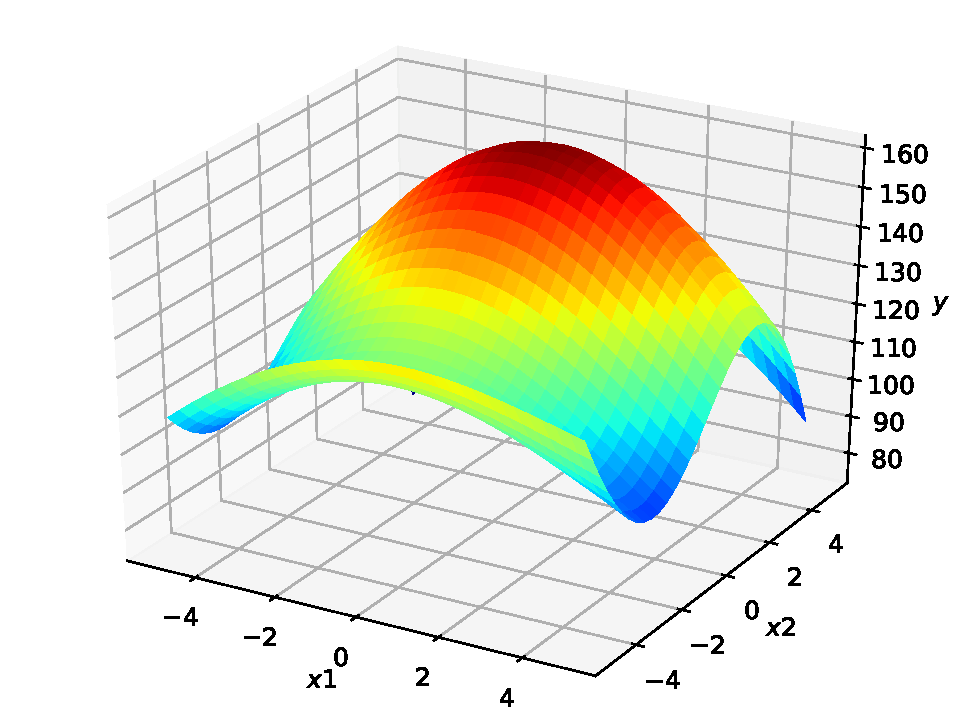
\includegraphics[width=0.47\linewidth]{tatiane/fig_tati/func_leo/fig3_ga_li.pdf}\label{a}}
	\subfigure[][]{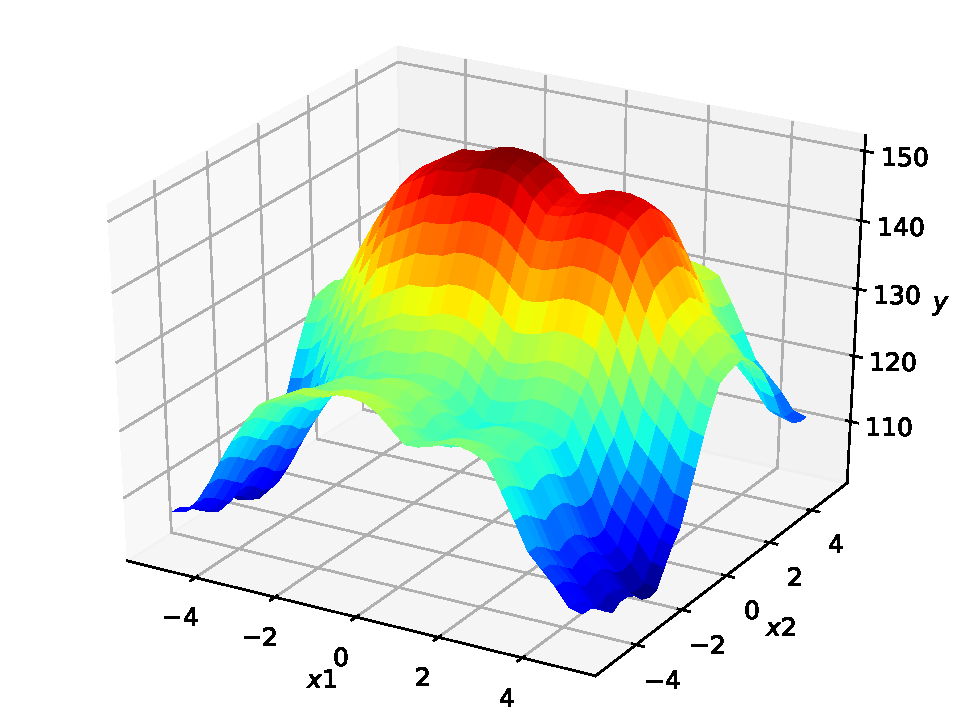
\includegraphics[width=0.47\linewidth]{tatiane/fig_tati/func_leo/fig4_lin_exp.pdf}\label{b}}
	\subfigure[][]{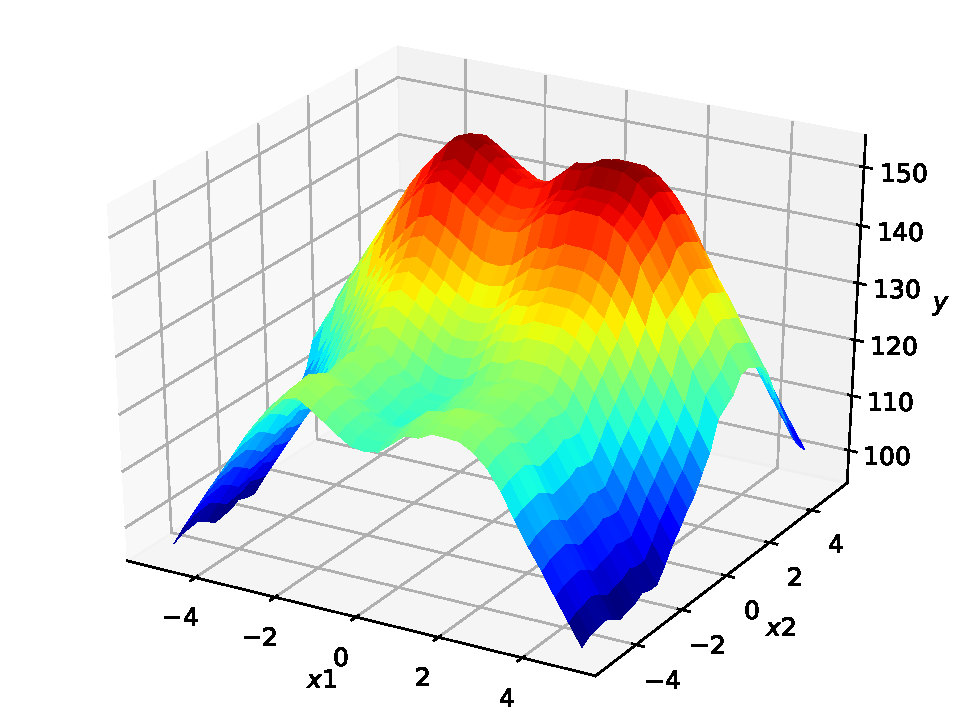
\includegraphics[width=0.47\linewidth]{tatiane/fig_tati/func_leo/fig5_exp_SQ.pdf}\label{c}}
	\subfigure[][]{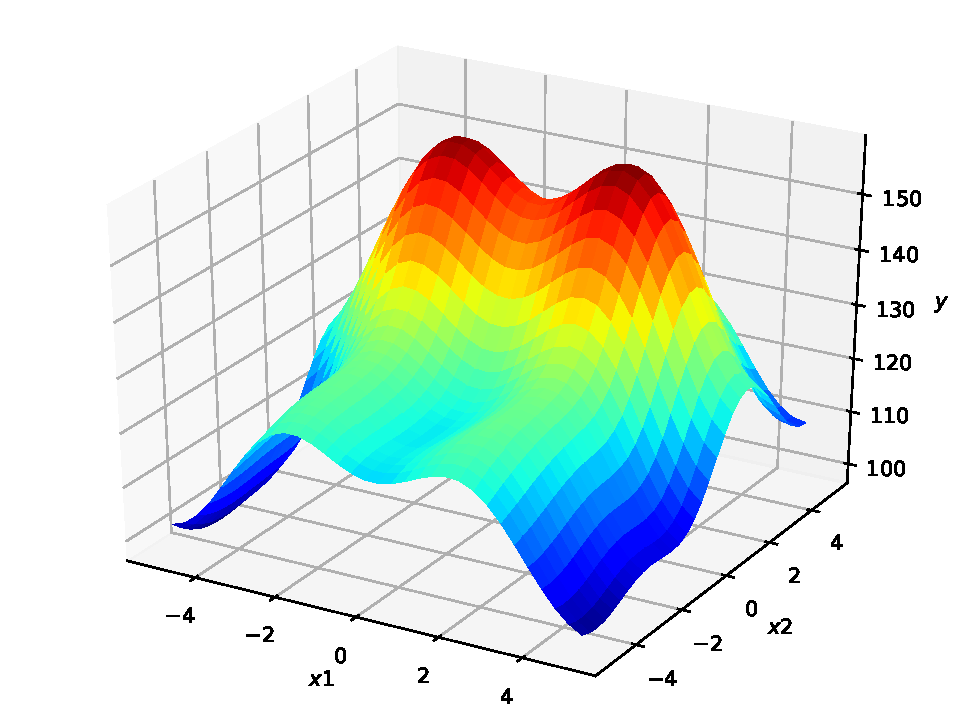
\includegraphics[width=0.47\linewidth]{tatiane/fig_tati/func_leo/fig6_rbf_con.pdf}\label{d}}
	\subfigure[][]{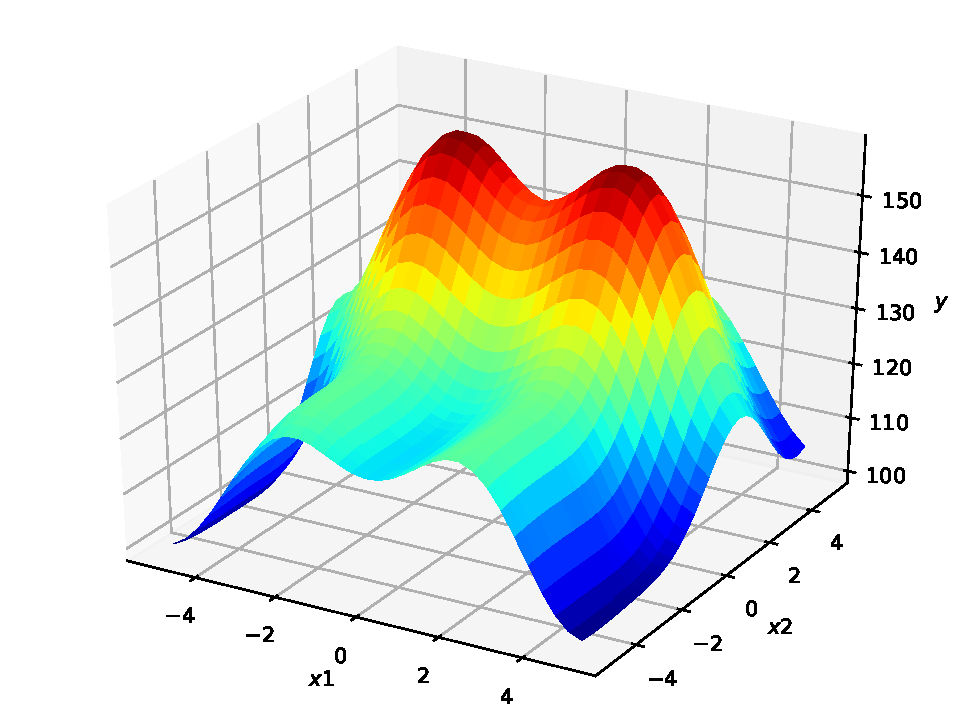
\includegraphics[width=0.47\linewidth]{tatiane/fig_tati/func_leo/fig7_rbf_con.pdf}\label{e}}
	\subfigure[][]{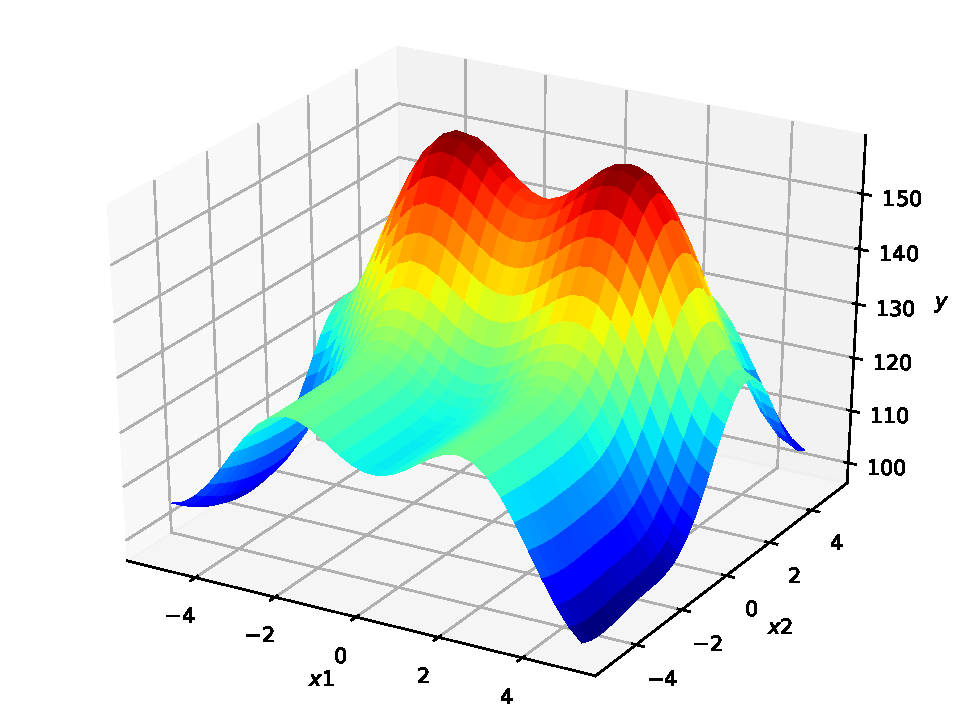
\includegraphics[width=0.47\linewidth]{tatiane/fig_tati/func_leo/fig8_rbf_lin.pdf}\label{f}} 
	\caption{Melhores configurações para a função quadrática: a) UK-LIN-GAUSS para 10 amostras; b) UK-LIN-EXP para 20 amostras; c) UK-SG-EXP para 30 amostras; d) RBF-C-GAUSS para 40 amostras; e) RBF-C-GAUSS para 50 amostras; f) RBF-LIN-GAUSS para 60 amostras.} 
	\label{fig:fl}
\end{figure}


Note que a forma da função é adequadamente representada a partir de 40 amostras geradas pelo LHS. Existe uma dificuldade dos metamodelos em descrever o comportamento da função quadrática para os valores maiores de $y$, além das extremidades da função. No entanto, essa dificuldade diminui \textcolor{red}{à} medida que um maior número de amostras é utilizado para a  formulação dos metamodelos considerados.

\section{Função \textit{Eggholder}}

Uma vez que as duas funções matemáticas descritas apresentaram uma boa precisão, escolheu-se como função de teste a {\it eggholder}. Esta função é largamente utilizada para testar algoritmos de otimização por possuir vários mínimos locais \cite{YONDO}. A função \textit{eggholder} é dada por:
\begin{equation}
y=-\left({x_2}+47\right)\sen\left(\sqrt{\left|\frac{x_1}{2}+({x_2}+47)\right|}\right)-\left({x_1}\sen\left(\sqrt{\left|{x_1}-({x_2}+47)\right|}\right)\right)
\end{equation}

\noindent onde $x_1 \in [-512, \hspace{0.1 cm}512]$ e  $x_2 \in [-512, \hspace{0.1 cm}512]$. A Fig. \ref{fig:eggholder} mostra o comportamento da função {\it eggholder} dentro do intervalo de amostragem definido.

\begin{figure}[H]
	\centering
	{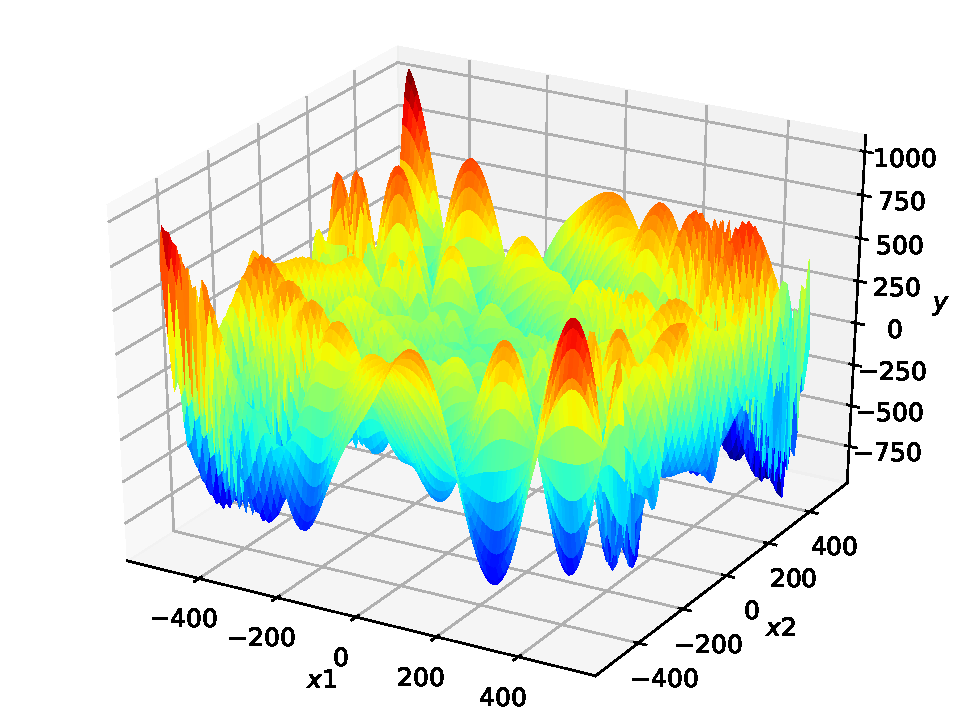
\includegraphics[width=0.65\linewidth]{tatiane/fig_tati/eggholder/fig2_eggholder.pdf}} 	
	\caption{Função \textit{eggholder}.} 
	\label{fig:eggholder}
\end{figure}

Devido à complexidade da função {\it eggholder}, 100, 200, 300, 400, 500 e 600 amostras foram geradas pelo método LHS para treinamento dos metamodelos. As mesma configurações admitidas para as funções Branin-Hoo e quadrática foram utilizadas para este caso. As Tabs. \ref{tab:7} e \ref{tab:8} apresentam os resultados obtidos a partir dos métodos {\it Kriging} e RBF. A Fig. \ref{fig:egg2} mostra o comportamento dos melhores metamodelos obtidos para a função \textit{eggholder}.\\

\begin{table}[H]
	\centering
	\caption{Métricas de precisão para a função \textit{eggholder} considerando 100, 200 e 300 amostras.} \label{tab:7} 
	\begin{tabular}{c c c c c c c c c}
		\toprule
		& \multicolumn{2}{c}{\bf 100 amostras} & \multicolumn{2}{c}{\bf 200 amostras} & \multicolumn{2}{c}{\bf 300 amostras} \\ \midrule
		{\bf Metamodelo} & RMSE & {\bf $R^{2}$} & RMSE & {\bf $R^{2}$} & RMSE & {\bf $R^{2}$} \\
		\hline \\[2pt] 
		{OK-GAUSS} & 258.4125 & 0.362013 & 241.9145 & 0.440875 & 176.9406 &	0.700884 \\[4pt]
		OK-EXP & 277.1001 &	0.266402 & 262.4458 & 0.341943 & 213.8278 &	0.563169   \\[4pt]                 
		UK–LIN-GAUSS & 269.2196 & 0.307535 & 243.6457 & 0.432844 & 177.2017 & 0.700000   \\[4pt]
		UK–LIN-EXP & 289.2422 &	0.200704 & 264.1655 & 0.333290 & 213.9439 &	0.562695    \\[4pt]
		UK–SG-GAUSS & 274.4885 & 0.280165 & 245.2200 & 0.425492  & 179.1079 &	0.693511   \\[4pt]
		UK–SG-EXP & 294.6476 & 0.170550 & 265.8468 & 0.324776 & 216.8872 &	0.550580   \\[4pt]
		RBF-C-GAUSS & 288.8072 & 0.203106 & 282.3682 &	0.238244 & 246.7164 &	0.418459  \\[4pt]
		RBF-LIN-GAUSS & 297.9746 & 0.151713 & 284.9116 & 0.224459 & 247.0129 & 0.417060  \\[4pt] \bottomrule
		
	\end{tabular}
	
\end{table}


\begin{table}[H]
	\centering
	\caption{Métricas de precisão para a função \textit{eggholder} considerando 400, 500 e 600 amostras.} \label{tab:8} 
	\begin{tabular}{c c c c c c c c c}
		\toprule
		& \multicolumn{2}{c}{\bf 400 amostras} & \multicolumn{2}{c}{\bf 500 amostras} & \multicolumn{2}{c}{\bf 600 amostras} \\ \midrule
		{\bf Metamodelo} & RMSE & {\bf $R^{2}$} & RMSE & {\bf $R^{2}$} & RMSE & {\bf $R^{2}$} \\
		\hline \\[2pt] 
		{OK-GAUSS} & 194.0209 & 0.640349 & 253.5398 & 0.385846 & 192.8466 & 0.644689  \\[4pt]
		OK-EXP & 199.9785 & 0.617923 & 196.3735	& 0.631574 & 180.1333 &	0.689992    \\[4pt]                 
		UK–LIN-GAUSS & 193.5777 & 0.641990 & 255.1658 & 0.377944 & 167.3490	& 0.732434    \\[4pt]
		UK–LIN-EXP & 200.0021 &	0.617832 & 196.5256 & 0.631003 & 180.3185 &	0.689354     \\[4pt]
		UK–SG-GAUSS & 195.1105 & 0.636297 & 259.1708 & 0.358263 & 168.4835 &	0.728794   \\[4pt]
		UK–SG-EXP & 200.0965 & 0.617472 & 197.1635 & 0.628604 & 181.4505 &	0.685442    \\[4pt]
		RBF-C-GAUSS & 241.5345 & 0.442631 & 232.6289 &	0.482975 & 221.2047 &	0.532509   \\[4pt]
		RBF-LIN-GAUSS & 243.7271 & 0.432465 & 233.7774 & 0.477857 & 221.8479 &	0.529786   \\[4pt] \bottomrule
		
	\end{tabular}
	
\end{table}

\begin{figure}[H]
	\centering
	\subfigure[][]{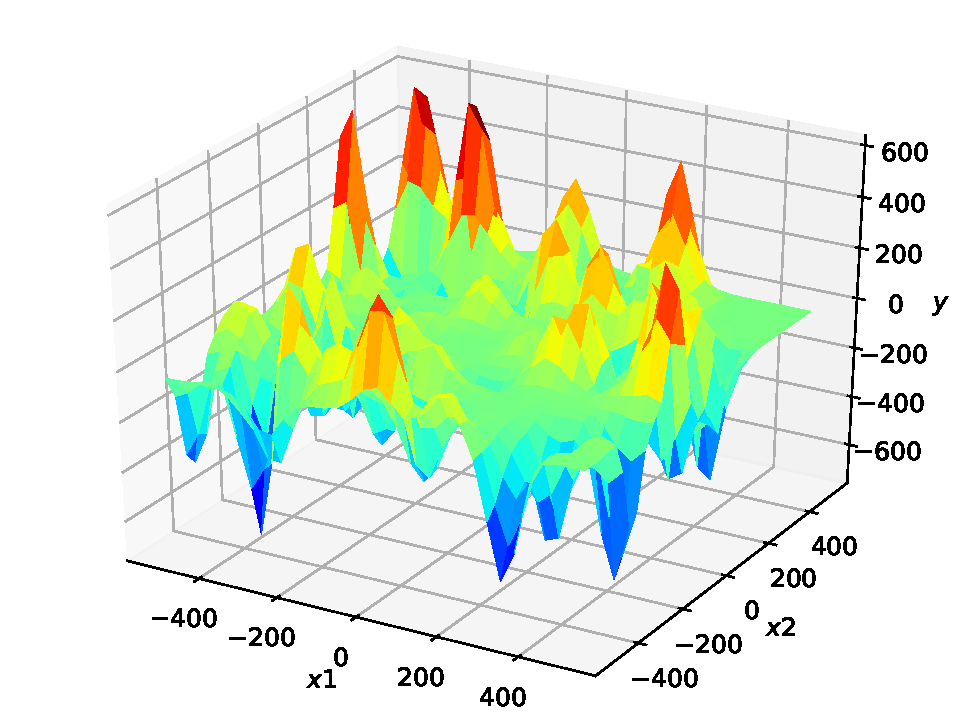
\includegraphics[width=0.47\linewidth]{tatiane/fig_tati/eggholder/fig3_ok_g.pdf}\label{a}}
	\subfigure[][]{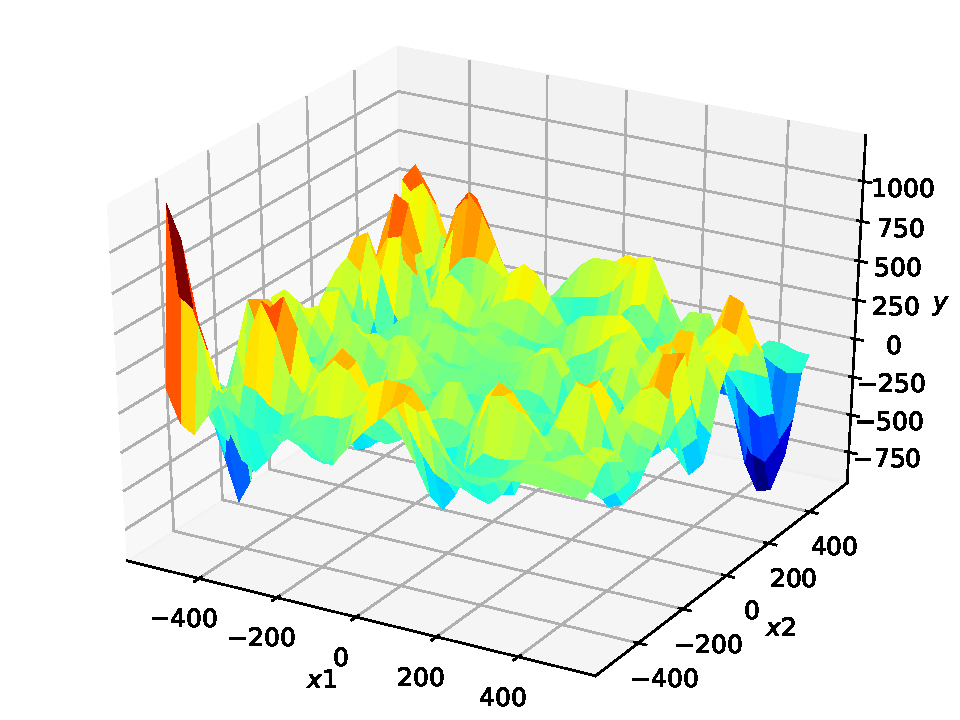
\includegraphics[width=0.47\linewidth]{tatiane/fig_tati/eggholder/fig4_ok_g.pdf}\label{b}}
	\subfigure[][]{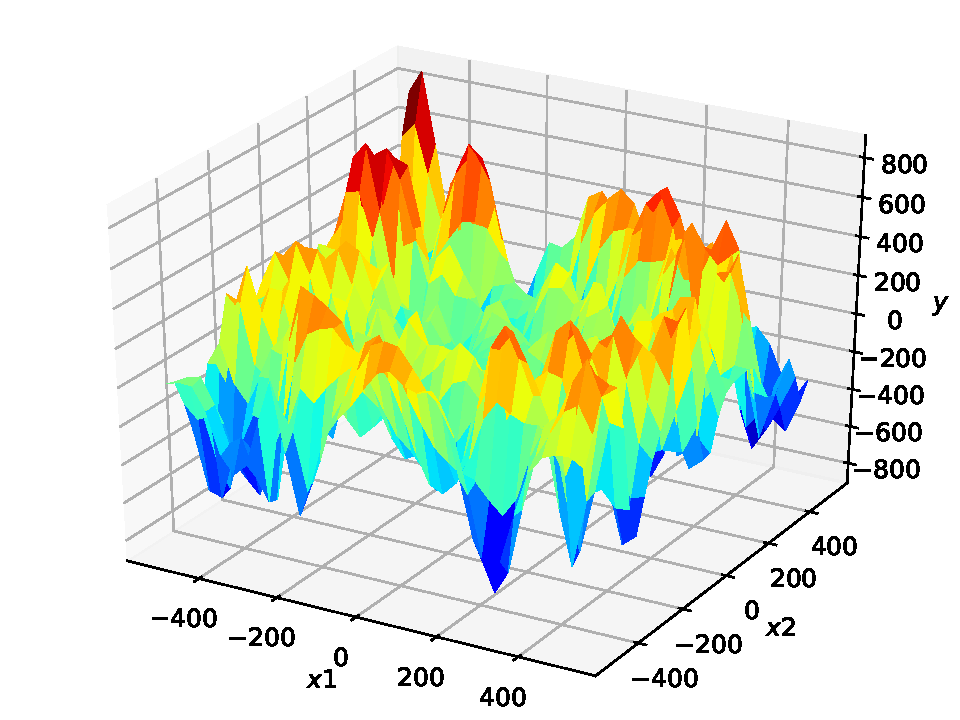
\includegraphics[width=0.47\linewidth]{tatiane/fig_tati/eggholder/fig5_ok_g.pdf}\label{c}}
		\subfigure[][]{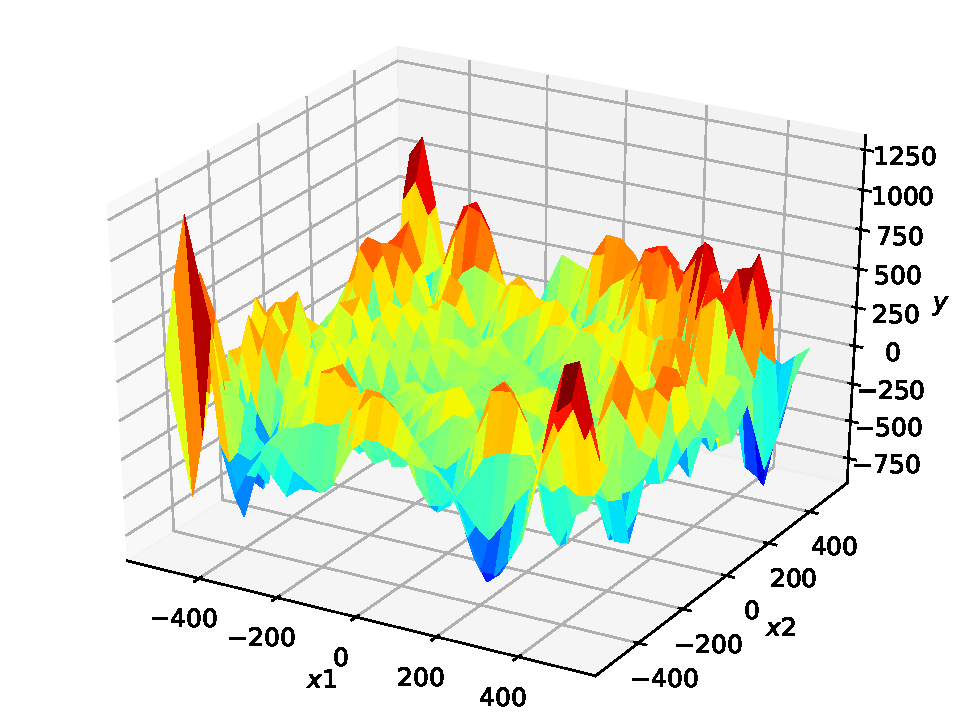
\includegraphics[width=0.47\linewidth]{tatiane/fig_tati/eggholder/fig6_lin_gaus.pdf}\label{d}}
	\subfigure[][]{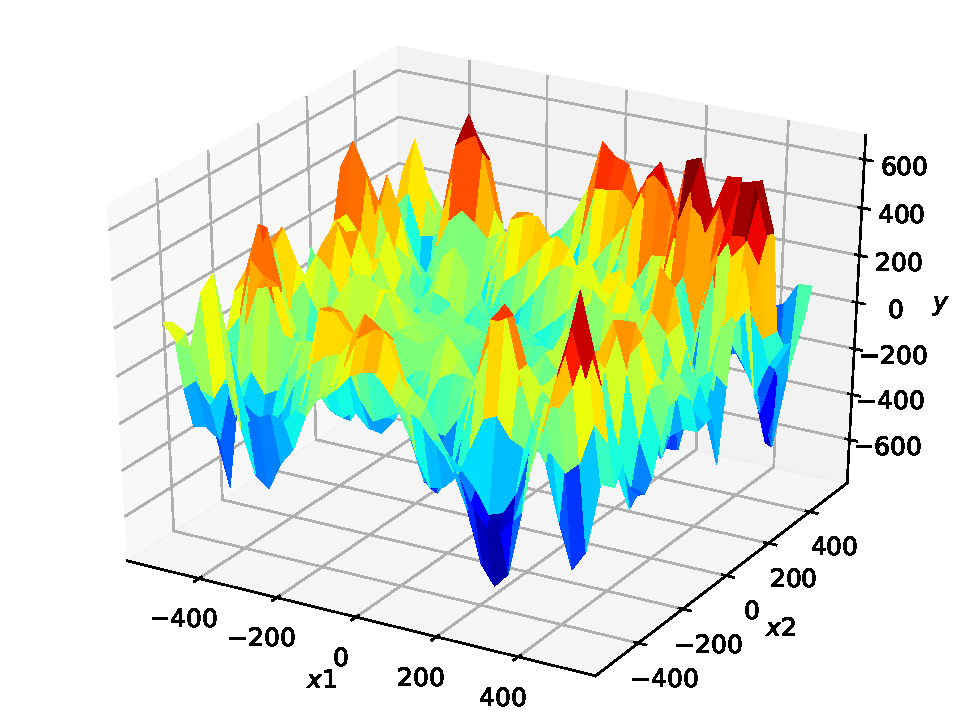
\includegraphics[width=0.47\linewidth]{tatiane/fig_tati/eggholder/fig7_ok_exp.pdf}\label{e}}
	\subfigure[][]{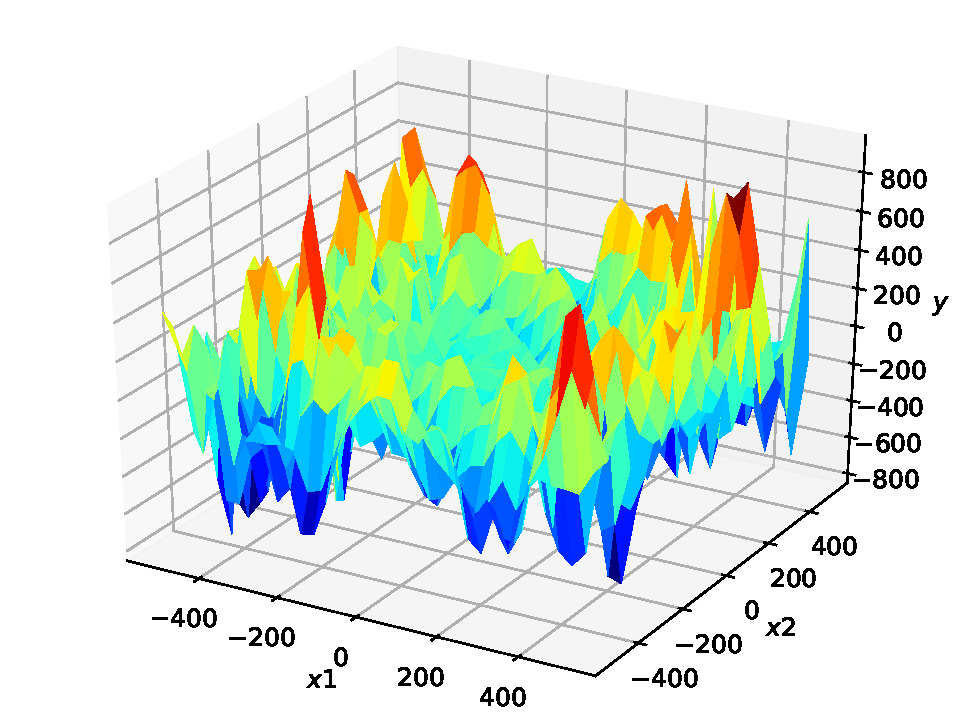
\includegraphics[width=0.47\linewidth]{tatiane/fig_tati/eggholder/fig8_lin_gaus.pdf}\label{f}}
	\caption{Melhores configurações para a função \textit{eggholder}: a) OK-GAUSS para 100 amostras; b) OK-GAUSS para 200 amostras; c) OK-GAUSS para 300 amostras; d) UK-LIN-GAUSS para 400 amostras; e) OK-EXP para 500 amostras; f) UK-LIN-GAUSS para 600 amostras.} 
	\label{fig:egg2}
\end{figure}

Como pode ser observado na Tab. \ref{tab:7}, os menores valores do RMSE e os valores mais próximos de 1 do ${R}^2$ para 100, 200 e 300 amostras foram obtidos pelo método OK-GAUSS. Para 600 amostras, o método se mostrou UK-LIN-GAUSS mais eficiente. Contudo, a representação da função \textit{eggholder} pelos metamodelos não se mostrou satisfatória. Os resultados obtidos são coerentes visto que, devido \textcolor{red}{à} complexidade da função {\it eggholder}, o número de amostras utilizado para o treinamento é insuficiente. 

É importante ressaltar que tentativas de treinamento com um maior número de amostras foram feitas. Contudo, para os metamodelos \textit{Kriging}, a matriz de correlação passou a ser não positiva-definida, impossibilitando a inversão da mesma. Isso acontece pelo mal condicionamento da matriz de correlação.

Um teste adicional\textcolor{red}{,} realizado com o objetivo de melhorar as respostas obtidas, modificando o método de otimização utilizado pelos metamodelos {\it Kriging}. Como mencionado, o pacote SMT considera o método COBYLA para minimizar a função dada pela Eq. (\ref{eq:35}). Assim, testou-se o método DE, sendo observada pouca melhora nas respostas obtidas.

Concluídas as discussões acerca da aplicação das referidas técnicas de amostragem e de metamodelagem em funções teste, partiu-se para o estudo de algumas destas metodologias no prolongamento de séries temporais. Tais análises serão discutidas a seguir.




\input{marcelo/anflex_surrogate_models}


Em relação aos testes realizados com as duas primeiras funções matemáticas, foram obtidos resultados satisfatórios. Em relação a função \textit{eggholder}, verifica-se que por ser uma função complexa e devido ao mal condicionamento da matriz de correlação, esta passou a não ser inversível para o metamodelo {\it Kriging} com função de correlação gaussiana. Assim, um estudo sobre outras maneiras de inverter a matriz de correlação será necessário como, por exemplo, utilizar a decomposição em valores singulares (SVD).

Observou-se que a precisão do metamodelo está relacionado com várias variáveis, como número de amostras para treinamento, distribuição das amostras no espaço de projeto, tipo de função polinomial, função de correlação e parâmetros que são fornecidos pelo projetista. Assim, uma alternativa discutida por \citeonline{viana2009} é utilizar uma combinação linear de metamodelos para melhorar a representatividade do modelo substituto final. 

Portanto, em relação ao trabalho desenvolvido na primeira etapa deste projeto de pesquisa, destaca-se a grande gama de metamodelos disponíveis no pacote SMT, onde alguns deles foram testados e resultados satisfatórios foram obtidos.

No entanto, através do trabalho realizado, foram identificadas várias oportunidades de estudo, como a combinação de diferentes metamodelos, o uso da validação cruzada para se determinar o melhor metamodelo, além da possibilidade de utilizar a Inferência Bayesiana, que tem ampla aplicação na consideração de incertezas. Claramente, faz parte dos estudos futuros a minimização do tempo computacional gasto para o metamodelo obtido estimar a solução do problema.   

